\section{Testing and Results}

After the model is trained, the next step is evaluating its performance and
testing it on new data. This section summarizes a lot of testing done on the
model and showcases some results obtained when experimenting with the parameter.
\newline
The main evaluation method to determine the performance of the model is plotting
its accuracy depending on the current epoch of the training. There are two kinds
of accuracies to measure, one performed on the training data and one on the
validation data. The validation accuracy is the more interesting one, as this
one is measured on data that the network hasn't seen yet.
\newline
The main parameters that were tested in this project, include the used model
itself, the size of the image, the used loss function and the number of epochs.
Additional parameters that could be experimented with would the ones defining
the specific layers in the model. To optimize those parameters the usage of a
tuner would be advised, as it can take a really long time to optimize them
manually. In the source code of this project one experimentation with such a
tuner can be found, due to time constraints this approach was not pursued any
further.
\newline
The model mentioned in the previous chapter was not the only one, that was
experimented with. The source code shows multiple different models that slightly
differ from each other in terms of number and order of layers. The vpp model is
one of the standards used in image classification with neural networks, which is
why the usage would have been preferred. Unfortunately the low computation power
of the laptops of all team members, the training of this model was not possible
in reasonable time. Therefore some slimed solutions were used:
\begin{figure}
    \centering
    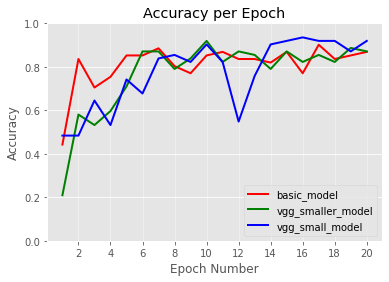
\includegraphics[width=0.4 \textwidth]{acc_per_epoch_models.png}
    \caption{validation accuracy of different models}
    \label{fig:models}
\end{figure}
As can be seen in figure \ref{fig:models} the performance of the different
models is quite similar. The validation accuracy goes up closely towards 90\%
which is a quite good performance considering the size and limit of the dataset.
Still the decision fell on the small vgg model, which is the one detailed in the
previous chapter. It has one break-in at epoch 12, where we will find the reason
for later.
\newline
The next parameter in question was the loss function. The three possibilities
here entailed the "categorical\_crossentropy", "mean\_square\_error" and
"mean\_squared\_logarithmic\_error". The first one is a recommended function to
be used with the classification of multiple classes. The mse (Mean Squared
Error) is generally used to approach the actual value as close as possible,
especially effective when the values are very close to each other. In comparison
the msle (Mean Squared Logarithmic Error) is very effective when values can lie
far apart from each other. Logically the msle should not make a lot of sense in
this context, but was used here to demonstrate a contrast.
\begin{figure}
    \centering
    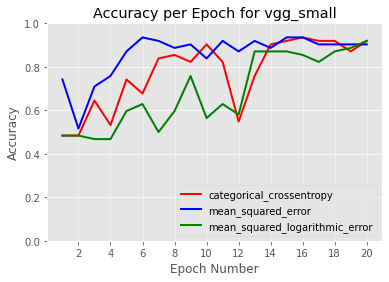
\includegraphics[width=0.4 \textwidth]{acc_per_epoch_loss.png}
    \caption{loss functions with small vgg}
    \label{fig:loss}
\end{figure}
Figure \ref{fig:loss} demonstrates exactly that. The msle takes the longest to
get to a good accuracy, while the other two functions are quicker, even though
they all eventually arrive at a similar accuracy. The highest ones where
achieved by the mse-function. Here a possible reason for the earlier noticed
break-in can be seen as well, as the entropy-function is the only one having
this same break-in and for the earlier tests, all models used this
loss-function. Still this could just be a coincidence because of a bad decision
made by the network.
\newline
For another more detailed comparison, Figure \ref{fig:mse} and Figure \ref{fig:msle} show all
relevant factors of both, the mse and msle. Here the difference can be clearly
seen.
\begin{figure}
\begin{subfigure}{.25\textwidth}
    \centering
    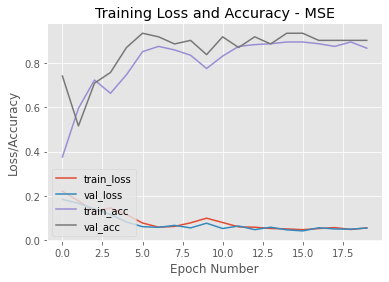
\includegraphics[width=0.9 \textwidth]{acc_per_epoch_mse.png}
    \caption{mse function}
    \label{fig:mse}
\end{subfigure}
\begin{subfigure}{.25\textwidth}
    \centering
    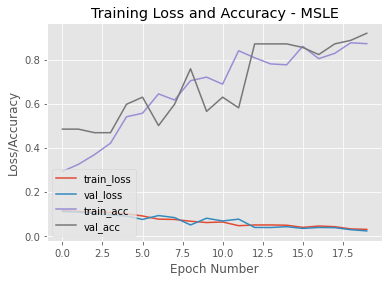
\includegraphics[width=0.9 \textwidth]{acc_per_epoch_msle.png}
    \caption{msle function}
    \label{fig:msle}
\end{subfigure}
\caption{two loss functions with small vgg}
\end{figure}
\newline
Another potential influence comes from the size of the image, as more detail
could mean a higher accuracy. As figure \ref{fig:size} shows, this might be
true, for images lower than 150 x 150 px, as you can still see a little trend
towards slower and more unstable progression. Looking at the difference between
180 x 180 px and 224 x 224 px, there is barely any. The 180px even seem to
slightly outperform the higher resolution, which in addition to longer computing
time, seem not the be worth the trouble.
\begin{figure}
    \centering
    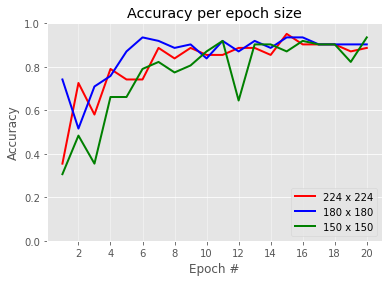
\includegraphics[width=0.4 \textwidth]{acc_per_epoch_size.png}
    \caption{different image sizes in px with small vgg}
    \label{fig:size}
\end{figure}
The final thing to do is finding a good number of epochs to train the network.
As figure \ref{fig:mse} shows our small vgg model with 180px and mse as loss
function, this graph represents the numbers we should focus on. The validation
accuracy here already hits a hight after five epochs and afterwards drops
slightly but staying mostly steady. It looks as if the network is already
satisfied after just a few epochs and further ones don't improve a lot. This
might be due to the small dataset or in general the limitation of having only
three different persons shown in the data.
\newline
This concludes the best settings for our model to be a 180 x 180 px image, using
the small vgg model with a mse-loss-function and going up to at least 5 epochs,
maybe a few more for good measure.
\newline
All these test where made with the classification of three different labels,
"no\_mask", "op\_mask" and "ffp2". This decision was made, as the fourth class
is very ambiguous especially in a small dataset, as it summarizes multiple masks
in one class. To not leave out the possibility of adding this last class, figure
\ref{fig:four} shows the performance of this network classifying all four classes.
\begin{figure}
    \centering
    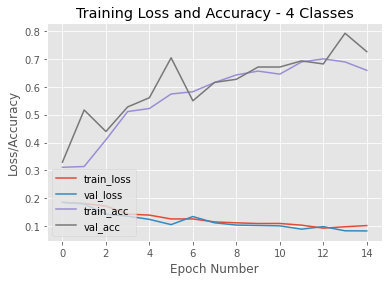
\includegraphics[width=0.4 \textwidth]{acc_per_epoch_four_classes.png}
    \caption{four classes with best parameters}
    \label{fig:four}
\end{figure}
\newline
Out of interest, the here used dataset using only images labeled as "no\_mask"
and "ffp2", was used in another model found online. The code was written by
Adrian Rosebrock and uses the already pre-trained MobilNetV2 classifier
\cite{Rosebrock2020}. This would be the goto implementation in case one is focused
on making the classifier work and not creating one from scratch. The advantage
is, that this classifier has already been trained on a lot of different images,
which allows it to much easier adjust weights for new purposes as long as it
involves image classification. Repurposing this for a simple mask / no mask
detection is very easy and very accurate. Listing 2 and Figure
\ref{fig:mobilenetv2} show the performance of this model. It is very clear, that
the performance is exceptional considering the training and validation data. It
would remain to be seen, how the model performs on new images with very
different faces, but it is clear to say, that this model outperforms the one
created in this project by far.

\lstinputlisting[language=md,breaklines,caption={classification report},captionpos=b]{../code/classification_mobilenetv2.md}

\begin{figure}
    \centering
    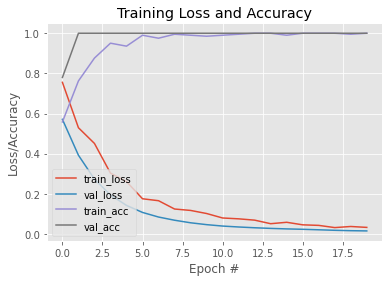
\includegraphics[width=0.4 \textwidth]{mobilenetv2_loss_and_acc.png}
    \caption{MobilNetV2 classifier - training results}
    \label{fig:mobilenetv2}
\end{figure}
